\documentclass[svgnames,
               hyperref={colorlinks,citecolor=DeepPink4,linkcolor=FireBrick,urlcolor=Maroon},
               usepdftitle=false]  % see \hypersetup{} below
               {beamer}

\mode<presentation>{
  \usetheme{Madrid}
  %\usecolortheme{seagull}
  \usecolortheme{seagull}
  \setbeamercovered{transparent}
  \setbeamerfont{frametitle}{size=\large}
}

\setbeamercolor*{block title}{bg=red!10}
\setbeamercolor*{block body}{bg=red!5}

%\usepackage[svgnames]{xcolor}
\usepackage{hyperref}
\hypersetup{
    pdftitle = {Toward nonlinear multigrid for nonlinear variational inequalities},
    pdfauthor = {Ed Bueler},
    pdfsubject = {},
    pdfkeywords = {}
}

\usepackage[english]{babel}
\usepackage[latin1]{inputenc}
\usepackage{times}
\usepackage[T1]{fontenc}
\usepackage{empheq,bm,xspace,fancyvrb,soul}
\usepackage{tikz}
\usetikzlibrary{shapes,arrows.meta,decorations.markings,decorations.pathreplacing,fadings,positioning}
\usepackage[kw]{pseudo}
\pseudoset{left-margin=15mm,topsep=5mm,idfont=\texttt,st-left=,st-right=}

\makeatletter
%\newcommand\notsotiny{\@setfontsize\notsotiny\@vipt\@viipt}
\newcommand\notsotiny{\@setfontsize\notsotiny\@viipt\@viiipt}
\makeatother

\newcommand{\eps}{\epsilon}
\newcommand{\RR}{\mathbb{R}}

\newcommand{\grad}{\nabla}
\newcommand{\Div}{\nabla\cdot}
\newcommand{\trace}{\operatorname{tr}}

\newcommand{\hbn}{\hat{\mathbf{n}}}

\newcommand{\bb}{\mathbf{b}}
\newcommand{\be}{\mathbf{e}}
\newcommand{\bbf}{\mathbf{f}}
\newcommand{\bg}{\mathbf{g}}
\newcommand{\bn}{\mathbf{n}}
\newcommand{\br}{\mathbf{r}}
\newcommand{\bu}{\mathbf{u}}
\newcommand{\bv}{\mathbf{v}}
\newcommand{\bw}{\mathbf{w}}
\newcommand{\bx}{\mathbf{x}}

\newcommand{\bF}{\mathbf{F}}
\newcommand{\bQ}{\mathbf{Q}}
\newcommand{\bU}{\mathbf{U}}
\newcommand{\bV}{\mathbf{V}}
\newcommand{\bX}{\mathbf{X}}

\newcommand{\btau}{\bm{\tau}}
\newcommand{\bxi}{\bm{\xi}}

\newcommand{\bzero}{\bm{0}}

\newcommand{\rhoi}{\rho_{\text{i}}}

\newcommand{\ip}[2]{\left<#1,#2\right>}

\newcommand{\mR}{R^{\bm{\oplus}}}
\newcommand{\iR}{R^{\bullet}}

\newcommand{\nn}{{\text{n}}}
\newcommand{\pp}{{\text{p}}}
\newcommand{\qq}{{\text{q}}}
\newcommand{\rr}{{\text{r}}}

\newcommand{\bus}{\bu|_s}
\newcommand{\oo}[1]{\displaystyle O\left(#1\right)}
\newcommand{\sold}{s_{\text{o}}}


\title[Multigrid for nonlinear VI]{Toward nonlinear multigrid \\ for nonlinear variational inequalities}

%\subtitle{\emph{x}}

\author{Ed Bueler}

\institute[UAF]{University of Alaska Fairbanks}

\date[]{February 2023}

%\titlegraphic{\begin{picture}(0,0)
%    \put(0,180){\makebox(0,0)[rt]{\includegraphics[width=4cm]{figs/software.png}}}
%  \end{picture}
%}

\titlegraphic{\hfill 
\includegraphics[width=0.15\textwidth]{images/uafbw.png}}

%% to start section counter at 0 see
%% https://tex.stackexchange.com/questions/170222/change-the-numbering-in-beamers-table-of-content


\begin{document}
\beamertemplatenavigationsymbolsempty

%\begin{frame}
%  \maketitle
%\end{frame}

{
  %\usebackgroundtemplate{\includegraphics[width=\paperwidth]{images/gray-british-clark2022.png}}
  \begin{frame}
    \titlepage
  \end{frame}
}

\begin{frame}{Outline}
  \tableofcontents[hideallsubsections]
\end{frame}


\section{variational inequalities (VIs)?}

\begin{frame}{example: a classical obstacle problem}

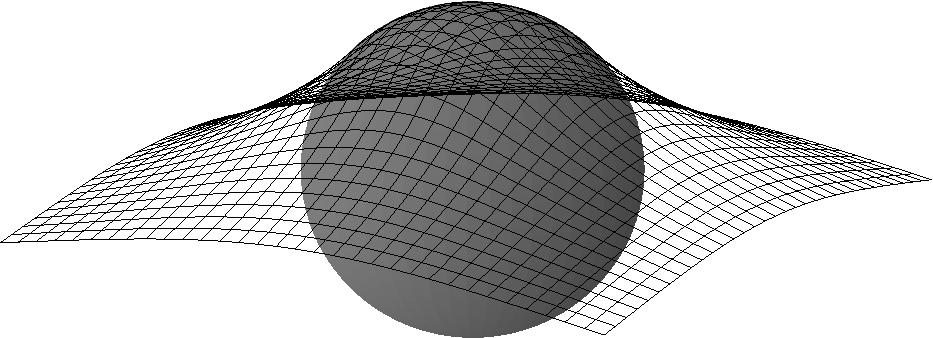
\includegraphics[width=0.6\textwidth]{images/obstacle65.pdf} \qquad 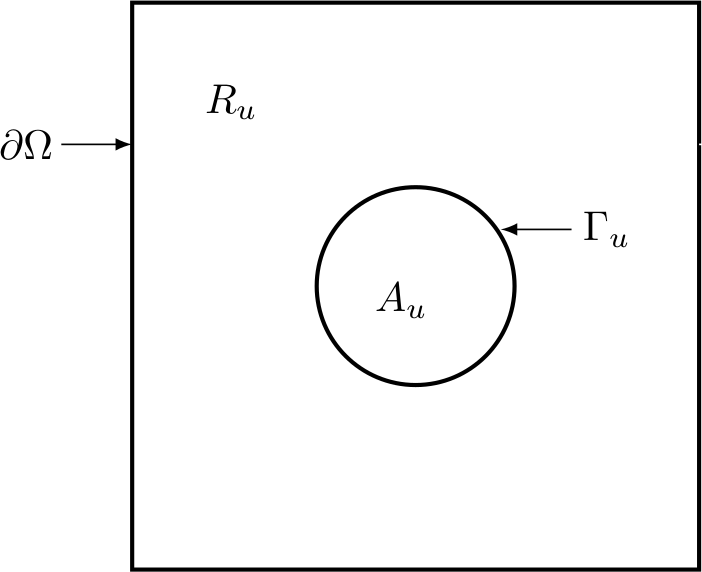
\includegraphics[width=0.3\textwidth]{images/obstacle-sets.png}

\bigskip
\only<1>{
\begin{itemize}
\item \emph{problem.} on a domain $\Omega \subset \RR^2$, find the displacement $u(x)$ of a membrane, with fixed value $u = g$ on $\partial \Omega$, above an \emph{obstacle} $\psi(x)$, which minimizes the elastic energy
    $$J(u) = \int_\Omega \frac{1}{2} |\grad u|^2 - f\, u$$
\item shown above: $\Omega=(-2,2)^2$, $\psi(x)$ a hemisphere
\end{itemize}
}
\only<2>{
\begin{itemize}
\item i.e.~constrained optimization over an \emph{admissible set}
	$$\mathcal{K} = \left\{v \in H^1(\Omega) \,:\, v\big|_{\partial \Omega} = g \text{ and } v \ge \psi\right\}$$
\item informally, $J'(u)$ points directly into $\mathcal{K}$ (\emph{variational inequality}; VI):
    $$\ip{J'(u)}{v-u} = \int_\Omega \grad u\cdot \grad (v-u) - f (v-u) \ge 0 \quad \text{for all } v \in \mathcal{K}$$
\end{itemize}
}
\only<3>{
\begin{itemize}
\item the solution defines \emph{active} $A_u = \{u = \psi\}$ and \emph{inactive} $R_u = \{u> \psi\}$ subsets of $\Omega$, and a \emph{free boundary} $\Gamma_u=\partial R_u \cap \Omega$
\item a naive strong form poses the problem in terms of its solution:
{\small
\begin{align*}
-\grad^2 u &= f \text{ on $R_u$} \\
u &= \psi \text{ on $A_u$}
\end{align*}
}
\item by contrast, the weak form VI is meaningful
\end{itemize}
}
\only<4>{
\begin{itemize}
\item a \emph{complementarity problem}, essentially KKT conditions, is a meaningful strong form:
{\small
\begin{align*}
u - \psi &\ge 0 \\
-\grad^2 u - f &\ge 0 \\
(u - \psi)(-\grad^2 u - f) &= 0
\end{align*}
}
\end{itemize}
}
\end{frame}


\begin{frame}{general VI problems}

\begin{itemize}
\item let $\mathcal{K}$ be a closed and convex subset of a Banach space $\mathcal{V}$
\item suppose $F:\mathcal{K} \to \mathcal{V}'$ is a continuous, generally nonlinear \emph{operator}
    \begin{itemize}
    \item[$\circ$] $F$ may be defined only on $\mathcal{K}$
    \end{itemize}
\item the general problem VI($F$,$\mathcal{K}$) is
	$$\ip{F(u)}{v-u} \ge 0 \text{ for all } v \in \mathcal{K}$$

\bigskip
\item analogy:

\begin{tabular}{l|l}
x & y \\ \hline
z & w
\end{tabular}
\end{itemize}
\end{frame}


\begin{frame}{Newton iterations for VIs}

\begin{columns}
\begin{column}{0.6\textwidth}
\begin{itemize}
\item x
\end{itemize}
\end{column}
\begin{column}{0.4\textwidth}
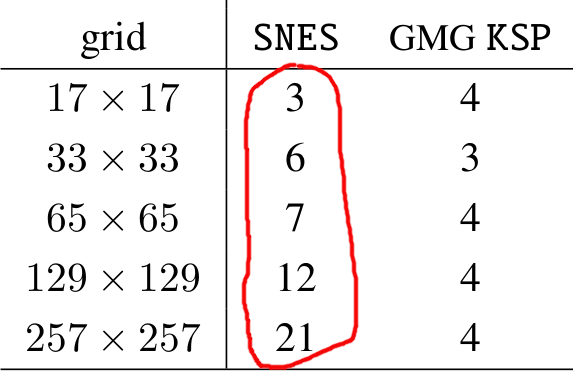
\includegraphics[width=\textwidth]{images/vi-newton-gmg-bad.png}

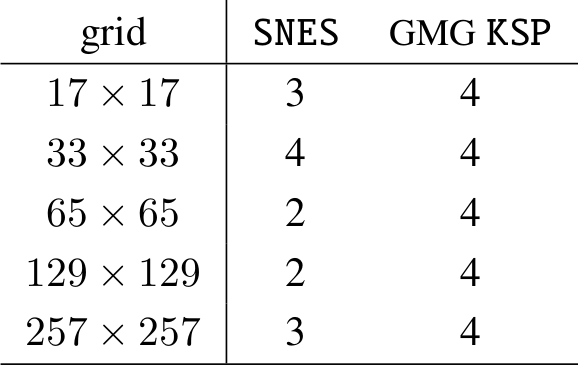
\includegraphics[width=\textwidth]{images/vi-newton-gmg-good.png}
\end{column}
\end{columns}
\end{frame}


\begin{frame}{Newton-multigrid for VIs}

xxx
\end{frame}


\begin{frame}{optimality}

\begin{columns}
\begin{column}{0.6\textwidth}
\begin{itemize}
\item x
\end{itemize}
\end{column}
\begin{column}{0.4\textwidth}
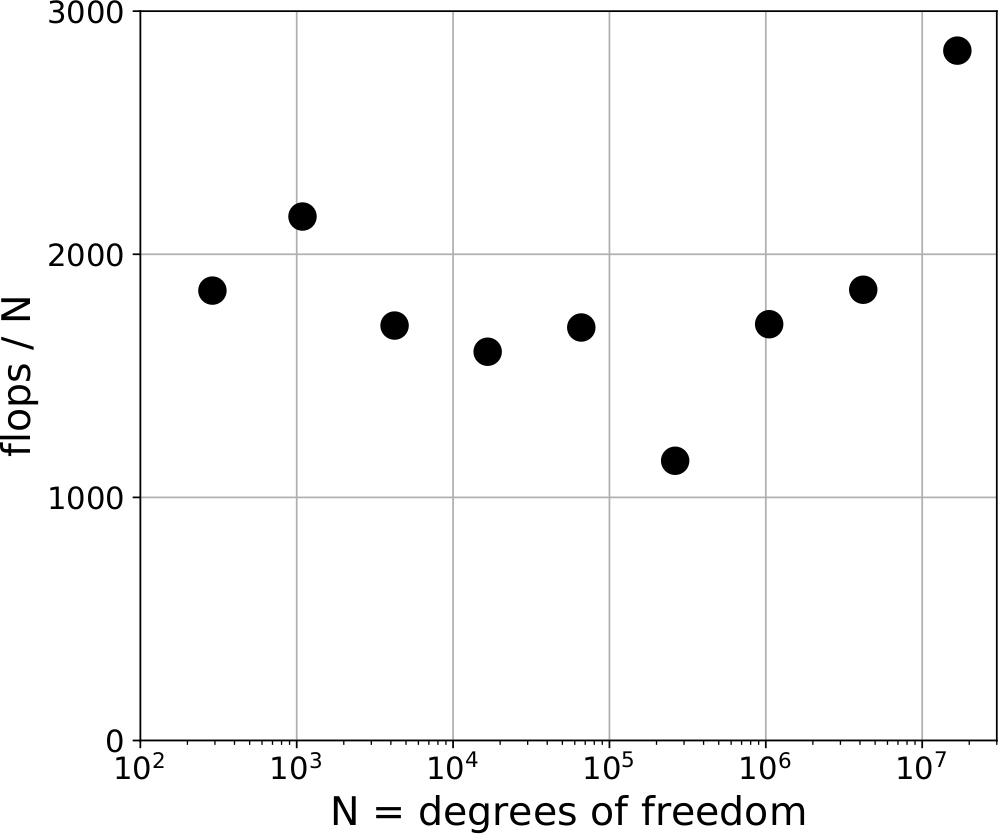
\includegraphics[width=\textwidth]{images/obstacle-flops-per-n.png}
\end{column}
\end{columns}
\end{frame}


\section{full approximation scheme (FAS) multigrid for PDEs?}

\begin{frame}{Bratu model problem: optimality}

\begin{columns}
\begin{column}{0.6\textwidth}
\begin{itemize}
\item x
\end{itemize}
\end{column}
\begin{column}{0.4\textwidth}
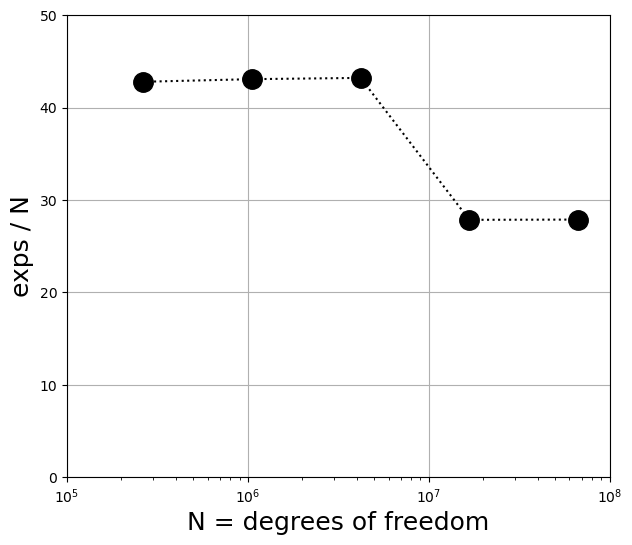
\includegraphics[width=\textwidth]{images/bratu-exps.png}

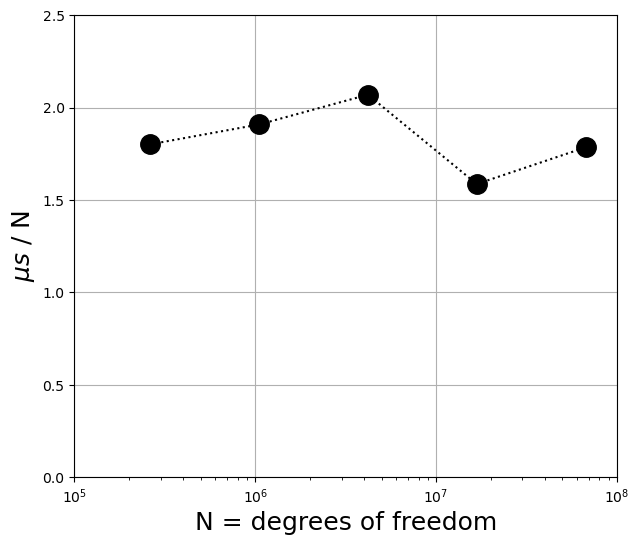
\includegraphics[width=\textwidth]{images/bratu-time.png}
\end{column}
\end{columns}
\end{frame}


\section{the nonlocal VI for a fluid layer in a climate}

\begin{frame}{problem: fluid layer in a climate}

\begin{center}
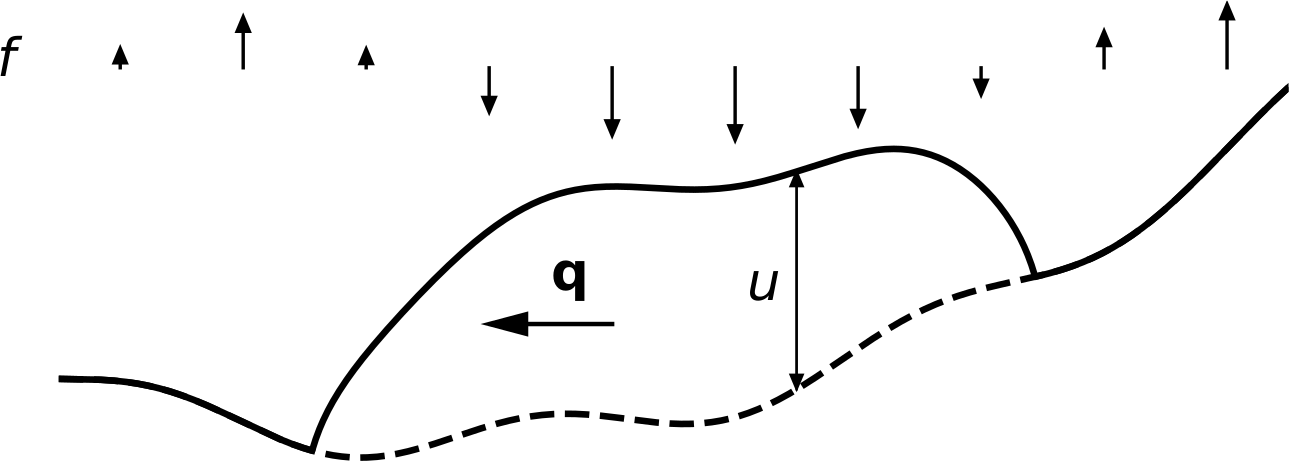
\includegraphics[width=0.6\textwidth]{images/fluid-in-climate.png}
\end{center}

\begin{itemize}
\item x
\end{itemize}
\end{frame}


\section{a possibly scalable approach to nonlocal VIs}


\begin{frame}{the Stokes problem for ice}

\begin{itemize}
\item whether explicit or implicit, a non-shallow model solves a Stokes problem at each step:
\begin{align*}
- \nabla \cdot \left(2 \nu_\eps(D\bu)\, D\bu\right) + \nabla p - \rhoi \mathbf{g} &= \bzero && \text{in $\Lambda$} \\
\nabla \cdot \bu &= 0 && \text{''} \\
\btau_b - \bbf(\bu|_b) &= \bzero && \text{on $\Gamma_b$} \\
\bu|_b \cdot \bn_b &= 0 && \text{''} \\
\left(2 \nu_\eps(D\bu) D\bu - pI\right) \bn &= \bzero && \text{on $\Gamma_s$}
\end{align*}
\item this is the \alert{stress balance} (conservation of momentum) problem which determines velocity $\bu$ and pressure $p$
\item how fast is the numerical solution process?
    \begin{itemize}
    \item[$\circ$] how do solution algorithms \alert{scale with increasing resolution}?
    \end{itemize}
\end{itemize}
\end{frame}




\begin{frame}{multilevel NCP-coupled-to-Stokes solvers}

\begin{itemize}
\item direct attack on the problem seems to require a \alert{multilevel} solver for \alert{variational inequalities} (VIs), but in the \alert{non-local residual case}
    \begin{itemize}
    \item[$\circ$] this seems not to exist
    \item[$\circ$] the \alert{smoother} must compute an implicit-step SKE residual including surface-motion term $\Phi(s) = - \bu|_s\cdot \bn_s$ from a scalable Stokes solver
    \end{itemize}
\item near-optimal multilevel VI solvers exist for toy problems
    \begin{itemize}
    \item[$\circ$] Poisson equation obstacle problem (Brandt \& Cryer 1983; Gr\"aeser \& Kornhuber 2009)
    \end{itemize}
\end{itemize}
\end{frame}


\section{conclusion}

\begin{frame}{\alert{summary}}

\begin{itemize}
\item x
\end{itemize}
\end{frame}


\begin{frame}{references}

{\scriptsize
%{\notsotiny
% inputed at end of slides.tex

\newcommand{\sdoi}[1]{\,{\tiny \href{https://doi.org/#1}{doi:#1}}}
\begin{itemize}
\item A.~Brandt \& C.~Cryer (1983). \emph{Multigrid algorithms for the solution of linear complementarity problems \dots}, SIAM J.~Sci.~Stat.~Comput.~4 (4), 655--684 \sdoi{10.1137/0904046}
%FTITLE Multigrid algorithms for the solution of linear complementarity problems arising from free boundary problems
\item P.~Brune, M.~Knepley, B.~Smith, \& X.~Tu (2015). \emph{Composing scalable nonlinear algebraic solvers}, SIAM Review~57 (4), 535--565 \sdoi{10.1137/130936725}
\item E.~Bueler (2021). \emph{Conservation laws for free-boundary fluid layers}, SIAM J.~Appl.~Math.~81 (5), 2007--2032 \sdoi{10.1137/20M135217X}
%\item E.~Bueler (2022). \emph{Performance analysis of high-resolution ice-sheet simulations}, J.~Glaciol., \sdoi{10.1017/jog.2022.113}
\item G.~de Diego, P.~Farrell, \& I.~Hewitt (2022). \emph{Numerical approximation of viscous contact problems applied to glacial sliding}, J.~Fluid Mech.~938 (A21). \sdoi{10.1017/jfm.2022.178}
\item P.~Farrell, M.~Croci, \& T.~Surowiec (2020). \emph{Deflation for semismooth equations}, Optimization Methods \& Software 35 (6), 1248--1271 \sdoi{10.1080/10556788.2019.1613655}
\item C.~Gr{\"a}ser \& R.~Kornhuber (2009). \emph{Multigrid methods for obstacle problems}, J.~Comput.~Math., 1--44
\item T.~Isaac, G.~Stadler, \& O.~Ghattas (2015). \emph{Solution of nonlinear Stokes equations \dots ice sheet dynamics}, SIAM J.~Sci.~Comput., 37 (6), B804--B833 \sdoi{10.1137/140974407}
%FTITLE Solution of nonlinear Stokes equations discretized by high-order finite elements on nonconforming and anisotropic meshes, with application to ice sheet dynamics
\item G.~Jouvet \& E.~Bueler (2012). \emph{Steady, shallow ice sheets as obstacle problems \dots}, SIAM J.~Appl.~Math.~72 (4), 1292--1314 \sdoi{10.1137/110856654}
%FTITLE Steady, shallow ice sheets as obstacle problems: well-posedness and finite element approximation
\item G.~Jouvet \& J.~Rappaz (2011). \emph{Analysis and finite element approximation of a nonlinear stationary {S}tokes problem \dots}, Adv.~Numer.~Analysis 2011 (164581) \sdoi{10.1155/2011/164581}
%FTITLE Analysis and finite element approximation of a nonlinear stationary {S}tokes problem arising in glaciology
\item R.~Kornhuber (1994). \emph{Monotone multigrid methods for elliptic variational inequalities I}, Numer.~Math.~69, 167--184 \sdoi{10.1007/BF03325426}
\item A.~Reusken (1987). \emph{Convergence of the multigrid full approximation scheme \dots}, Numer.~Math.~52, 251--277 \sdoi{10.1007/BF01398879}
%FTITLE Convergence of the multigrid full approximation scheme for a class of elliptic mildly nonlinear boundary value problems
\item J.~Seguinot \& 5 others (2018).  \emph{Modelling last glacial cycle ice dynamics in the Alps}, The Cryosphere, 12 (10), 3265--3285 \sdoi{10.5194/tc-12-3265-2018}
%FAUTHORS Seguinot, J., Ivy-Ochs, S., Jouvet, G., Huss, M., Funk, M., & Preusser, F.
\item X.~Tai (2003). \emph{Rate of convergence for some constraint decomposition methods for nonlinear variational inequalities}, Numer.~Math.~93 (4), 755--786 \sdoi{10.1007/s002110200404}
\end{itemize}


}
\end{frame}

\end{document}
